\scanpage{357}
\uline{Th Eilenberg-Zilber-Cartier}\hfill\mspage{EZ 1}

\(X_{**}\) un \deleted{groupe}\inserted{objet} abélien bisimplicial \((\qquad)\).
\deleted{\unsure{\(N\)} \unsure{bisimplicial}}
\[
\begin{aligned}
N &: A_{**}\xrightarrow[\sim]{\text{eq de cat}} A_{\bullet\bullet}\\
\text{(complexe associé}\quad \sim &: A_{**}\longrightarrow A_{\bullet\bullet}\\
\Delta &: A_{**}\longrightarrow A_*\\
\int &: A_{\bullet\bullet}\longrightarrow A_\bullet
\end{aligned}
\qquad
\begin{aligned}
N &: A_*\longrightarrow A_\bullet\\
\sim &: A_*\longrightarrow A_\bullet\\
N&\hookrightarrow \widetilde{(\ )}\quad\unsure{\text{q iso}}\\[-2pt]
&\hspace{4em}\uparrow\\[-2pt]
&\hspace{3.5em}D(\ )\quad\unsure{\text{degen homot triv}}
\end{aligned}
\]
\(\exists\) des \deleted{\unsure{quasi iso} naturels}\inserted{morphismes} fonctoriels,
\diagram{\begin{tikzcd}[ampersand replacement=\&]
\int N\arrow[r,shift right,"\varphi"'] \& N\Delta\arrow[l,shift right,"\psi"']
\end{tikzcd}}
\inserted{\(X_{0,0}\)} qui coincident avec les fleches evidentes en degré 0.
\diagram{\begin{tikzcd}[ampersand replacement=\&]
A_{**}\arrow[r,"N"]\arrow[d,"\Delta"'] \& A_{\bullet\bullet}\arrow[d,"\int"]\arrow[r,no head] \& {\deleted{\longrightarrow}}\\
A_*\arrow[r,"N"] \& A_\bullet\arrow[l,bend right,shorten >=1.5em,shorten <=1.5em]\arrow[l,bend left,shorten >=1.5em,shorten <=1.5em,<-] \&
\end{tikzcd}}
\[
\begin{aligned}
\varphi\psi&\sim1_{\unsure{\int N|N\Delta}}\\
\psi\varphi&\sim1_{\unsure{\int\Delta|N\Delta}}
\end{aligned}
\]
\(\deleted{\unsure{\varphi(X_{**})}}\)
\[
\begin{aligned}
\psi\varphi\quad\int (NX_{**})&\longrightarrow\int NX_{**}\\
\varphi\psi\quad N\Delta X_{**}&\longrightarrow N\Delta X_{**}\\
1-\psi\varphi&=dk+kd\qquad k:\int NX_{**}\xrightarrow{+1}\int NX_{**}\\
1-\varphi\psi&=dh+hd\qquad h:N\Delta X_{**}\xrightarrow{+1}N\Delta X_{**}
\end{aligned}
\]
\diagram{\begin{tikzcd}[ampersand replacement=\&]
\int N\arrow[r,shift left,"\psi"]\arrow[d] \& N\Delta\arrow[l,shift left,"\varphi"]\arrow[d]\\
\int\sim\arrow[r,shift left,"\widetilde\psi"] \& {\sim\Delta}\arrow[l,shift left,"\widetilde\varphi"]
\end{tikzcd}}
\diagram{\begin{tikzcd}[ampersand replacement=\&]
\int\sim\arrow[r,shift right,"\widetilde\varphi"'] \& {\sim(\Delta)}\arrow[l,shift right,"\widetilde\psi"']
\end{tikzcd}}
\deleted{\(k-k'=\)} Si \(\varphi\) et \(\psi\) sont choisis, Pour un autre choix de \(h',k'\)
\[
\begin{aligned}
k'-k&=dl+ld\\
h'-h&=dm+md
\end{aligned}
\quad\begin{aligned}&\text{etc \ldots}\\&l\ \text{et}\ m\ \text{fonct}\end{aligned}
\]

\deleted{EZ 2} \(\exists\) des choix traditionnels : \textquotedblleft application d'Alexander Whitney\textquotedblright{} \textquotedblleft shuffles\textquotedblright

\uuline{cf MacLane} Homology
\[
\begin{aligned}
\left(\int\widetilde X_{**}\right)_n&=\bigoplus_{i+j=n}X_{\unsure{(i)(j)|(i),(j)|(i,j)}}\xrightarrow{\text{shuffles}}\widetilde X_{(n,n)}\\
x_{ij}&\longrightarrow\deleted{\unsure{\sum\epsilon s_{\alpha}'s_{\beta}}}\quad x_{i+j,i+j}
\end{aligned}
\]
\((i,j)\)-shuffle \(\quad(1\ \ldots,\ \overset{\unsure{n\cdot|n}}{i+j})\)
\[
\begin{aligned}
&\hspace{12em}\unsure{\vert|1}\\
x_{i1}&\qquad x_{i+1,i+1}\qquad s(1)\ldots s(i)\quad s(i+j)\\
\sum_{0\leq a\leq i}(-1)^{\unsure{a}}s'_0s'_1\ldots\widehat{\unsure{s_a|s'_a|s_{\alpha}}}\ldots s'_i\,x_{i1}
&\qquad\sum_{\text{sur ttes }\sigma\in\Sigma_n}
s_{\sigma(i+1)}\ldots s_{\sigma(i+j)}\;s'_{\sigma(1)}\ldots s'_{\sigma(i)}
\end{aligned}
\]
\margin{Shuffles}\quad\unsure{signe|sgn}\((\sigma)\)
\[
\begin{aligned}
&\text{t.q }\sigma(\alpha)<\sigma(\beta)\\
&\alpha<\beta\leq i\quad\text{ou }\deleted{\unsure{i\leq}}\quad i<\alpha<\beta\leq n.\\
&\unsure{\sigma\in}
\end{aligned}
\]
\(A\qquad\overline B(A)\)
\figure{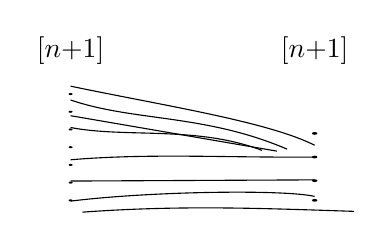
\begin{tikzpicture}[x=1cm,y=0.5cm]
\node at (0,3.8) {$[n\deleted{\unsure{+1}}]$};
\node at (3.1,3.8) {$[\unsure{n}\deleted{\unsure{+1}}]$};
\foreach \y in {0,0.45,0.9,1.35,1.8,2.25,2.7}
{\fill (0,\y) circle (.026);}\foreach \y in {0,.5,1.1,1.7}{\fill (3.1,\y) circle (.035);}
\draw (0,2.9) .. controls (1.2,2.4) and (2.5,2) .. (3.1,1.4);
\draw (0,2.55) .. controls (.8,2) and (1.7,2.2) .. (2.75,1.3);
\draw (0,2.15) -- (2.62,1.25);
\draw (0,1.85) .. controls (.7,1.58) and (1.6,1.9) .. (2.43,1.27);
\draw (0,1.03) .. controls (1,1.2) and (2,1.08) .. (3.1,1.1);
\draw (0,.49) -- (3.1,.52);
\draw (0,-.02) .. controls (1,.23) and (2.7,.28) .. (3.1,.1);
\draw (.15,-.3) .. controls (1.4,-.12) and (2.4,-.2) .. (3.6,-.28);
\end{tikzpicture}}

\uuline{Alexander-Whitney}
\[
\begin{aligned}
\widehat X_{n,n}&\longrightarrow\bigoplus X_{ij}\\
x_{n,n}&\longrightarrow\sum_{i=0}^{n}(-1)^i d_0^{n-i}\widehat{d'^{i}}x_{n,n}
\end{aligned}
\]
\diagram{\begin{tikzcd}[ampersand replacement=\&]
\underbrace{C^i(X,A)}_{f}\otimes\underbrace{C^j(X,B)}_{g}\arrow[r,Rightarrow] \& C^{i+j}(X\times X,A\otimes B)\arrow[dr] \&\\
\mathbb ZX\otimes\mathbb ZX \& \mathbb Z(X\times X)\arrow[l,Rightarrow] \& C^{i+j}(X,A\otimes B)
\end{tikzcd}}
\(\widehat{d}\) signifie le dernier op face

\(d'\) second op simpl.
\[
\widehat{d'^{i}}=d'^{n}d'^{n-1}\ldots d'^{n-i+1}
\]
\(EZ^{-1}\Rightarrow EZ\)

Cup-produit \(\left\{\begin{aligned}
&h(x_1,\ldots,x_{n+1})\\
&=\sum(-1)f(x_1,\ldots,x_i)g(x_{i+1},\ldots,x_n)
\end{aligned}\right.\)

\uline{Associatif}\quad (non-commutatif mais comm à homotopie près) \(\Rightarrow H^*(X,R)\) est anticom.
% archive sheet number: 358
